%
%
%
%
%
%
\section{Linear versus Non-linear Analysis}
\headb{Transonic Turbine Stage}{Linear versus non-linear analysis}
\label{linvnon_rt27.sec}
%
%
 An evaluation of whether non linearity could be responsible for discrepancies
 between the linear predicted results and measured data is presented in this
 section.
 A non-linear time-marching solution technique was employed to calculate the
 unsteady flow field in a coupled stator-rotor configuration. The stator to
 rotor pitch ratio is 3:5 thus three stator blades and five rotor blades have to
 be included in the computational domain.
 Because of the large number of point needed for a 3D calculation,
 the comparison beween linearised and non-linear methods was made using
 a quasi-3D version of the code at mid-height section.
%
%
%
%
\subsection{Analysis at mid-height section}
%
 Fig. \ref{rotor_mac_kul.fig} shows the predicted steady-state Mach number
 contours, using a quasi-3D representation,
 together with the Kulite sensor position.
 The isentropic Mach number blade distribution is compared with the time-averaged
 experimental data and the 3D calculation in Fig.
 \ref{rotor_blade_machis1.fig}.
%
%
\begin{figure}[ht]
   \centerline{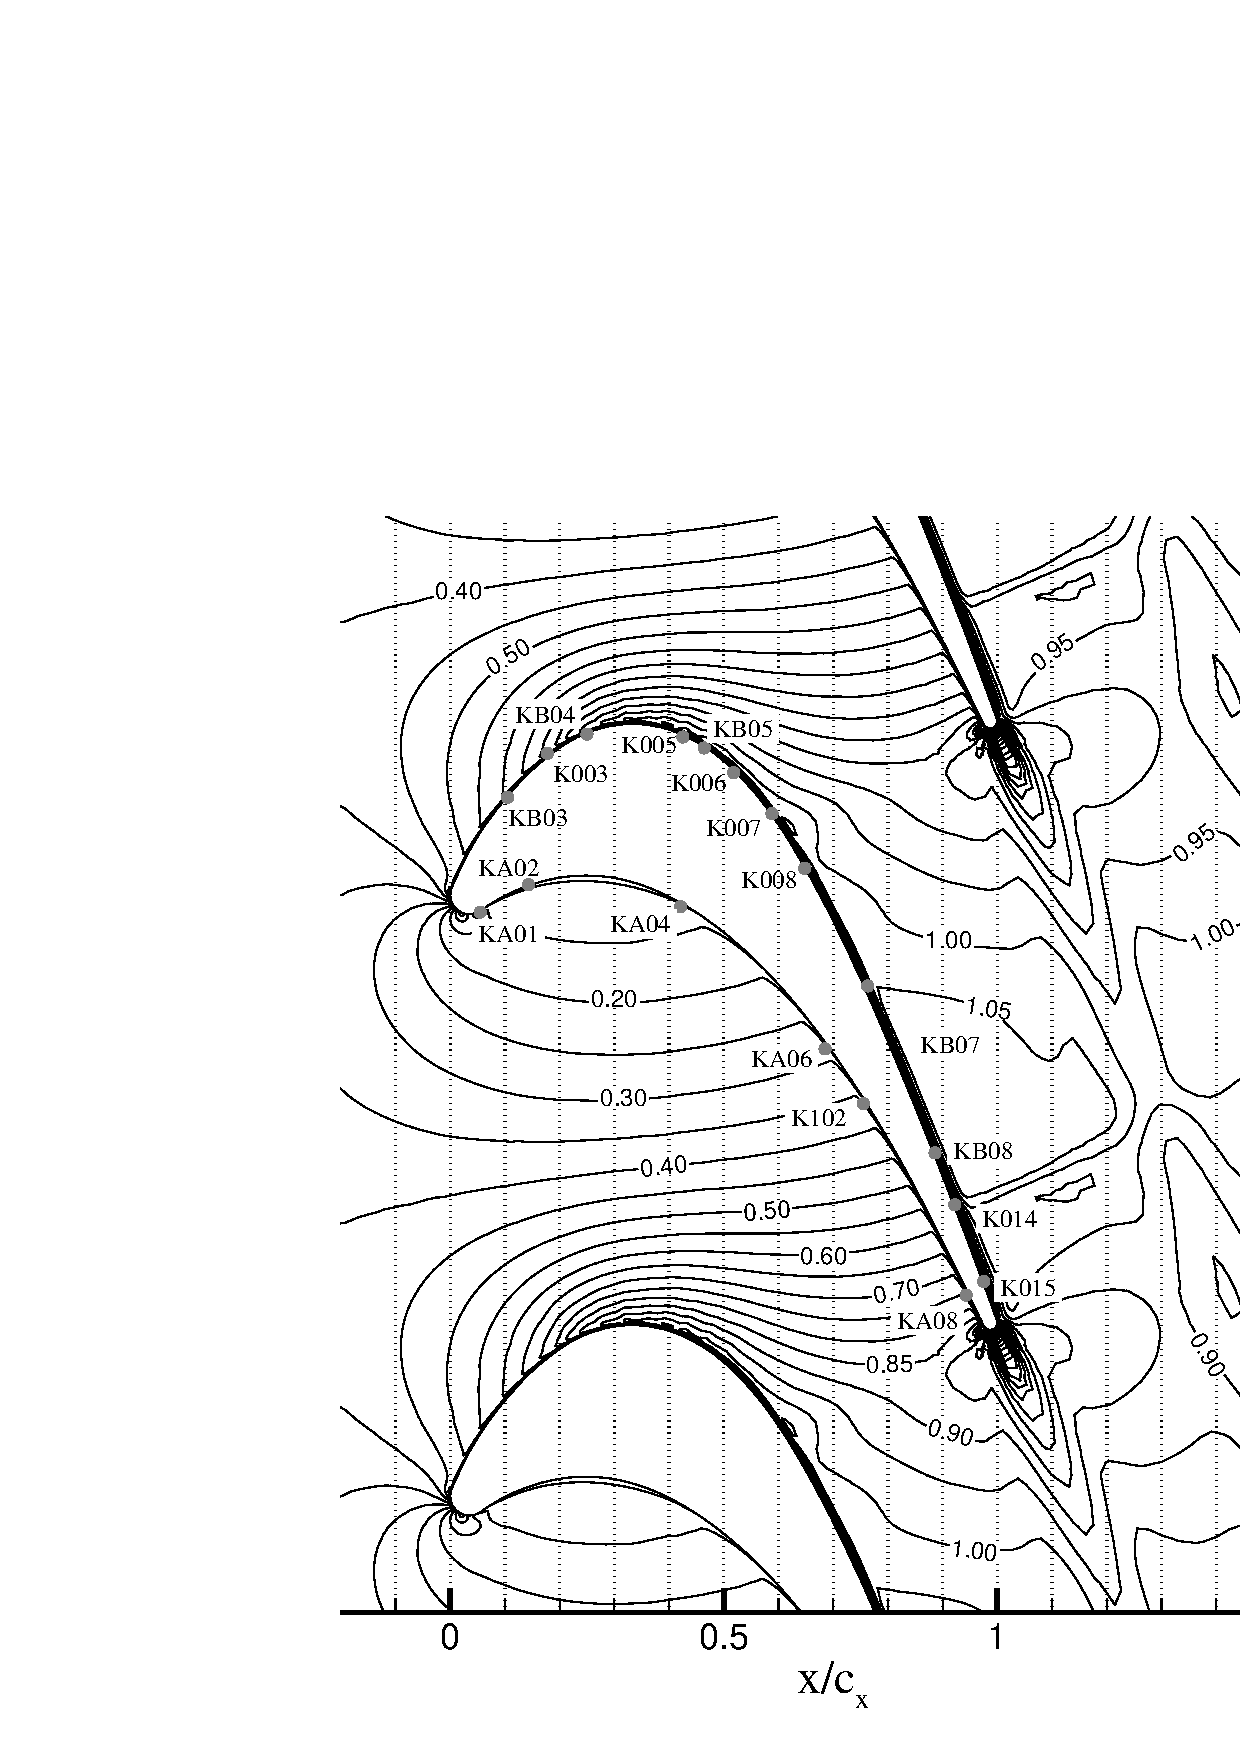
\includegraphics[width=100mm,clip=t]{CHAP_RT27/FIGURE/rot_mac_kul.pdf}}
   \caption{Steady-state Mach number contours on RT27a rotor mid-section
            and Kulite sensor position}
   \label{rotor_mac_kul.fig}
\end{figure}
%
%
 The non-linear time marching simulation for a coupled sistem of 3 NGV blades
 and 5 rotor blades run for eight blade frequency cicles before reaching a periodic
 solution suitable for comparison with the linear prediction.
 The unsteady pressure time-hystory on the rotor surface has been Fourier
 decomposed and the first three modes were considere.
 Higher Fourier components are strongly affected by the artificial
 diffusion/dispersion of the
 numerical algorithm (Sbardella \citeyearNP{Luca:2}).

 Figs. \ref{rt27_unsteady_1.fig}, \ref{rt27_unsteady_2.fig} and
 \ref{rt27_unsteady_3.fig} compare the results obtained using
 the linear and non-linear methods with
 the experimental data for the first three Fourier modes.
 For the first Fourier mode the discrepancies between linear and non-linear results
 are located in the leading-edge region of the blade. Such mismatch is maximum
 for $x\approx 0.35$ were linear perturbation is 50\% the non-linear one.
 In the pressure side and in the second part of the suction side the discrepancies
 are within a 10\% limit. On the other hand, the phase of the unsteady pressure
 perturbation is nearly the same for the linear and non-linear
 representations.
 The comparison between the linear and non-linear second Fourier component
 of Fig. \ref{rt27_unsteady_2.fig} indicates an even better agreement
 between the two representations. The error in amplitude prediction is well
 within a 10/\% limit. The phase is also in good agreement.
%
\begin{figure}
  \begin{flushleft}
   \begin{tabular}{ll}
     \subfigure[Amplitude of $\widetilde{p}/p_0$]
      {\hspace{-10mm}
       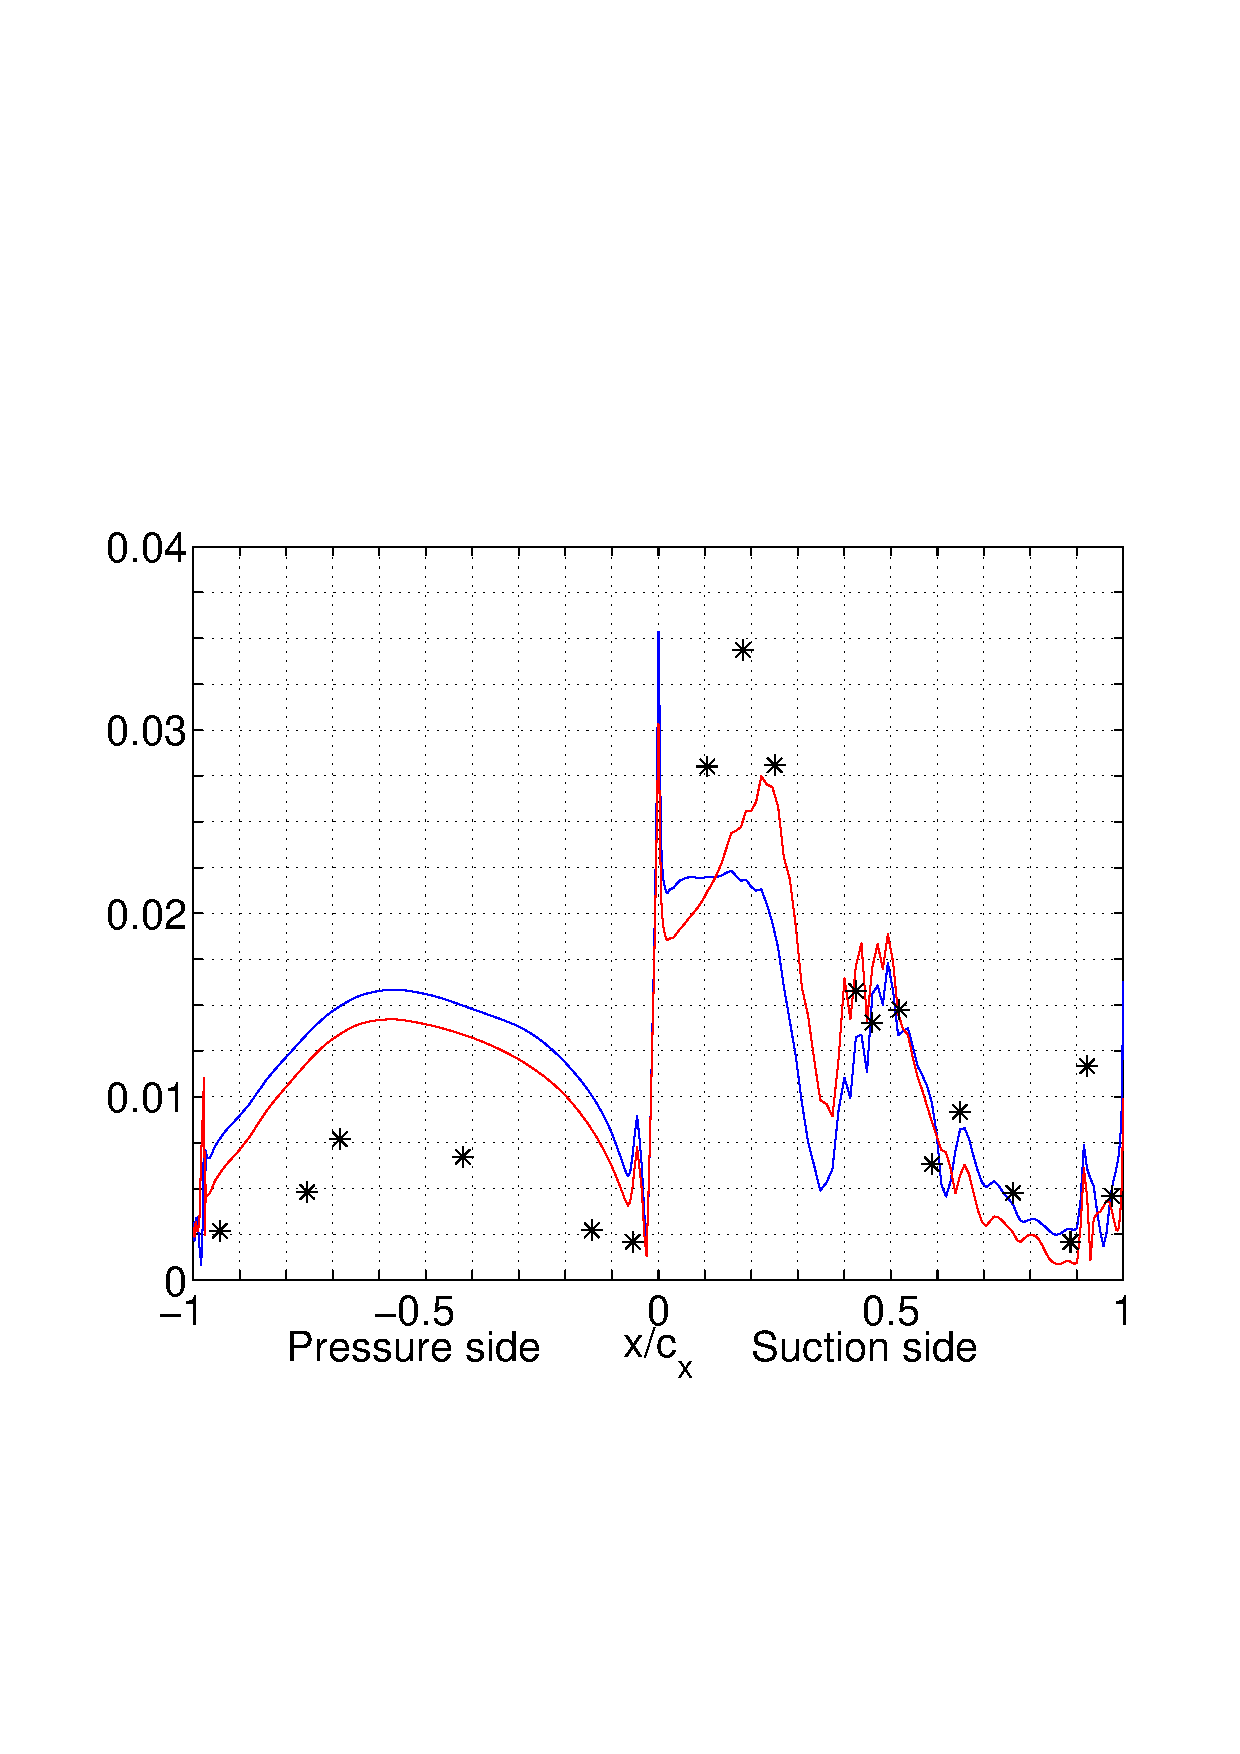
\includegraphics[width=75mm,clip=t]{CHAP_RT27/FIGURE/uns1amp1.pdf}}
         &
     \subfigure[Phase (deg)]
      {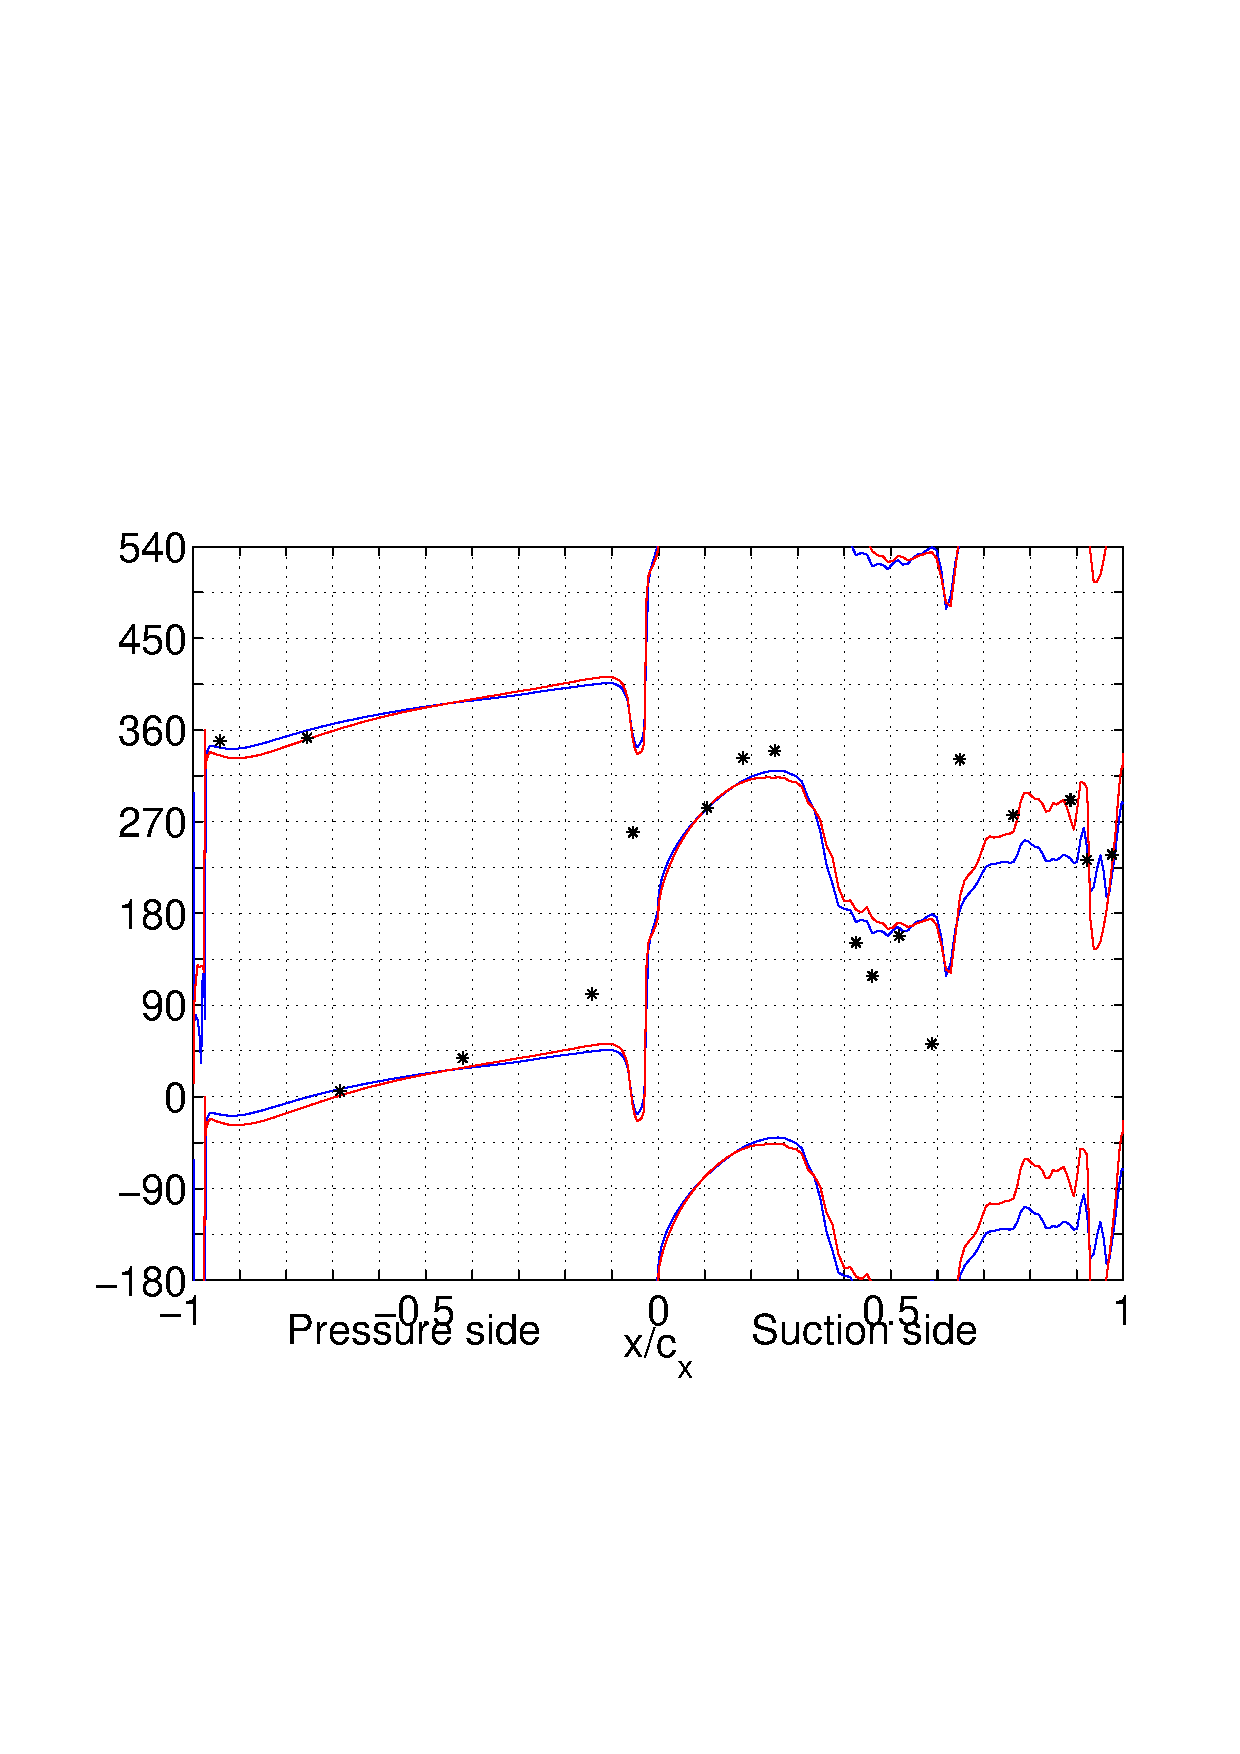
\includegraphics[width=75mm,clip=t]{CHAP_RT27/FIGURE/uns1pha1.pdf}}
   \end{tabular}
  \end{flushleft}
  \vspace{-8mm}
  \caption{RT27a rotor blade mid-section. First Fourier component of
           dimensionaless unsteady pressure.
           Linear method (blue),
           non-linear method (red) and
           measured data (stars).}
  \label{rt27_unsteady_1.fig}
\end{figure}
%
\begin{figure}
  \begin{flushleft}
   \begin{tabular}{ll}
     \subfigure[Amplitude of $\widetilde{p}/p_0$]
      {\hspace{-10mm}
       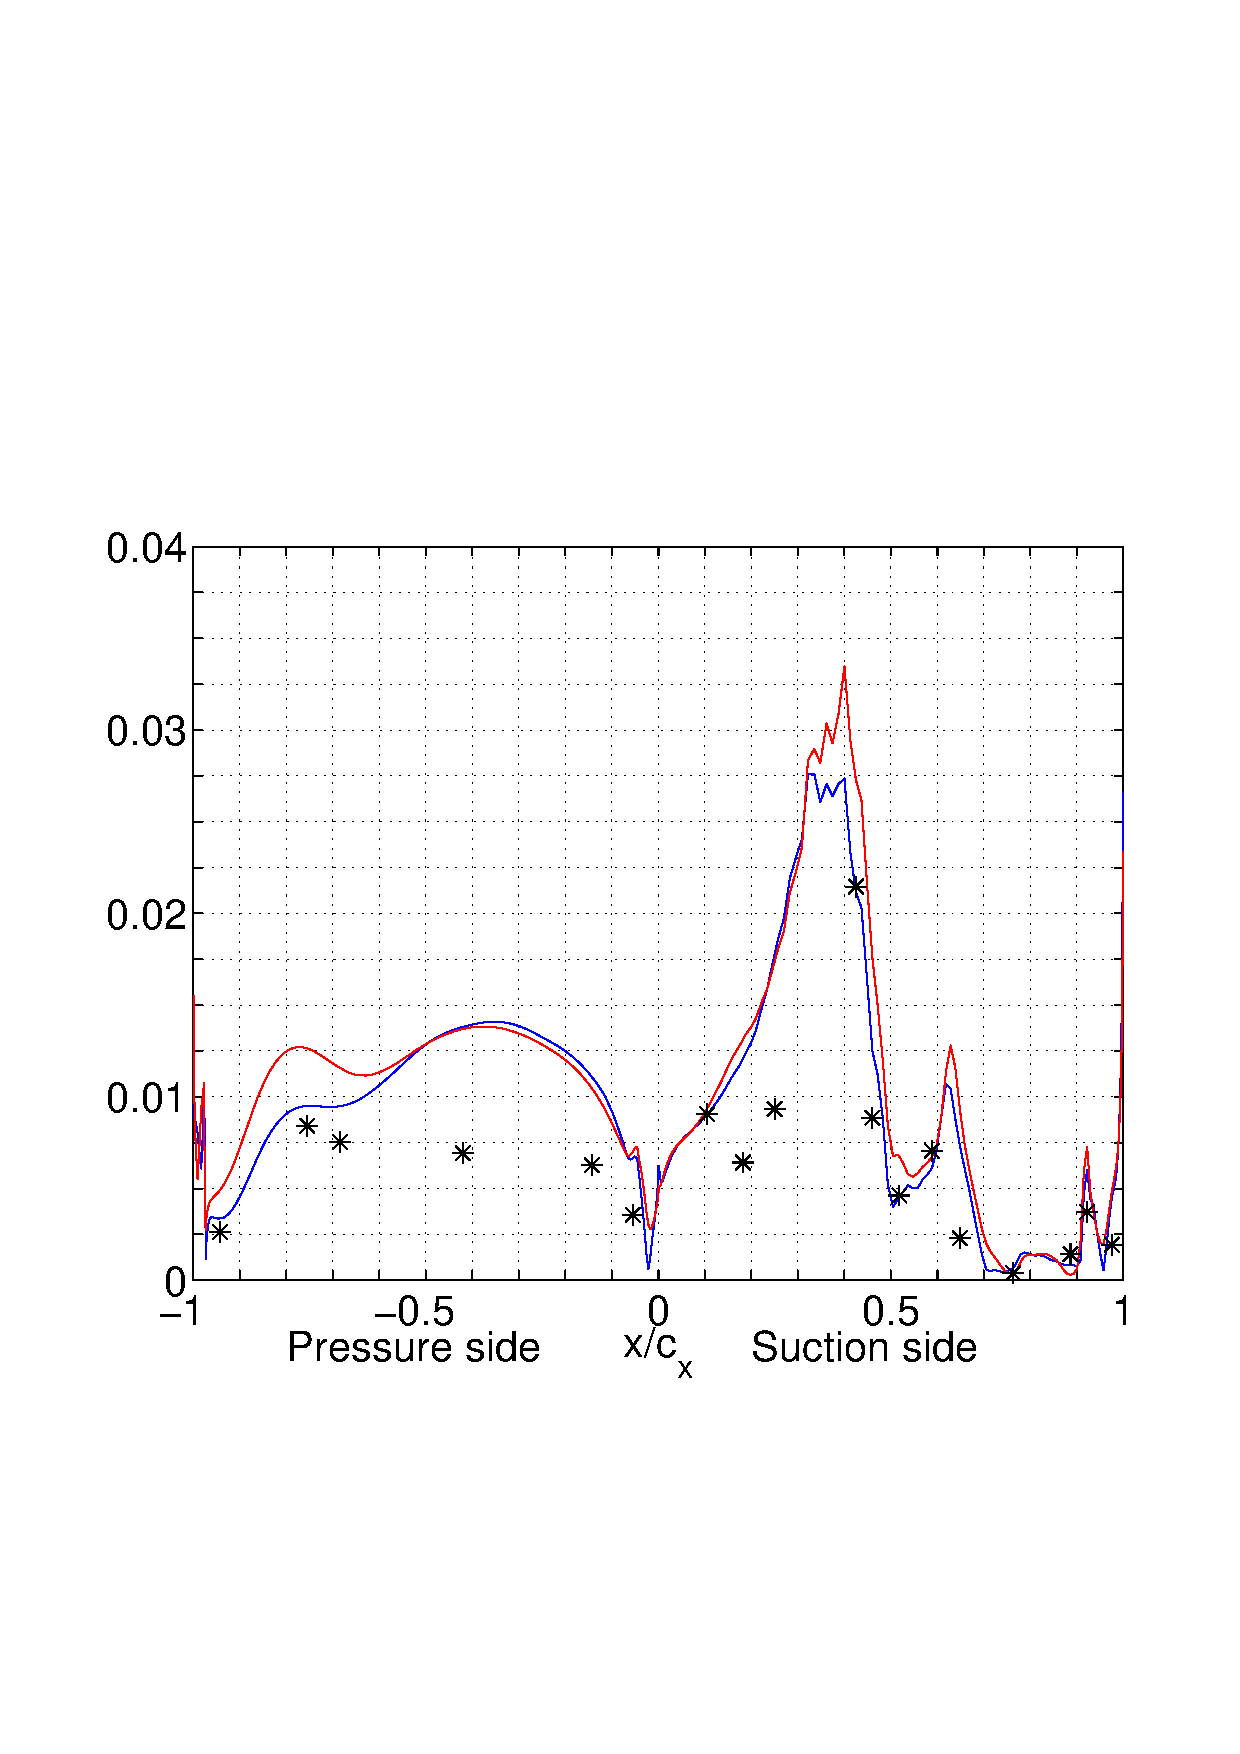
\includegraphics[width=75mm,clip=t]{CHAP_RT27/FIGURE/uns1amp2.pdf}}
         &
     \subfigure[Phase (deg)]
      {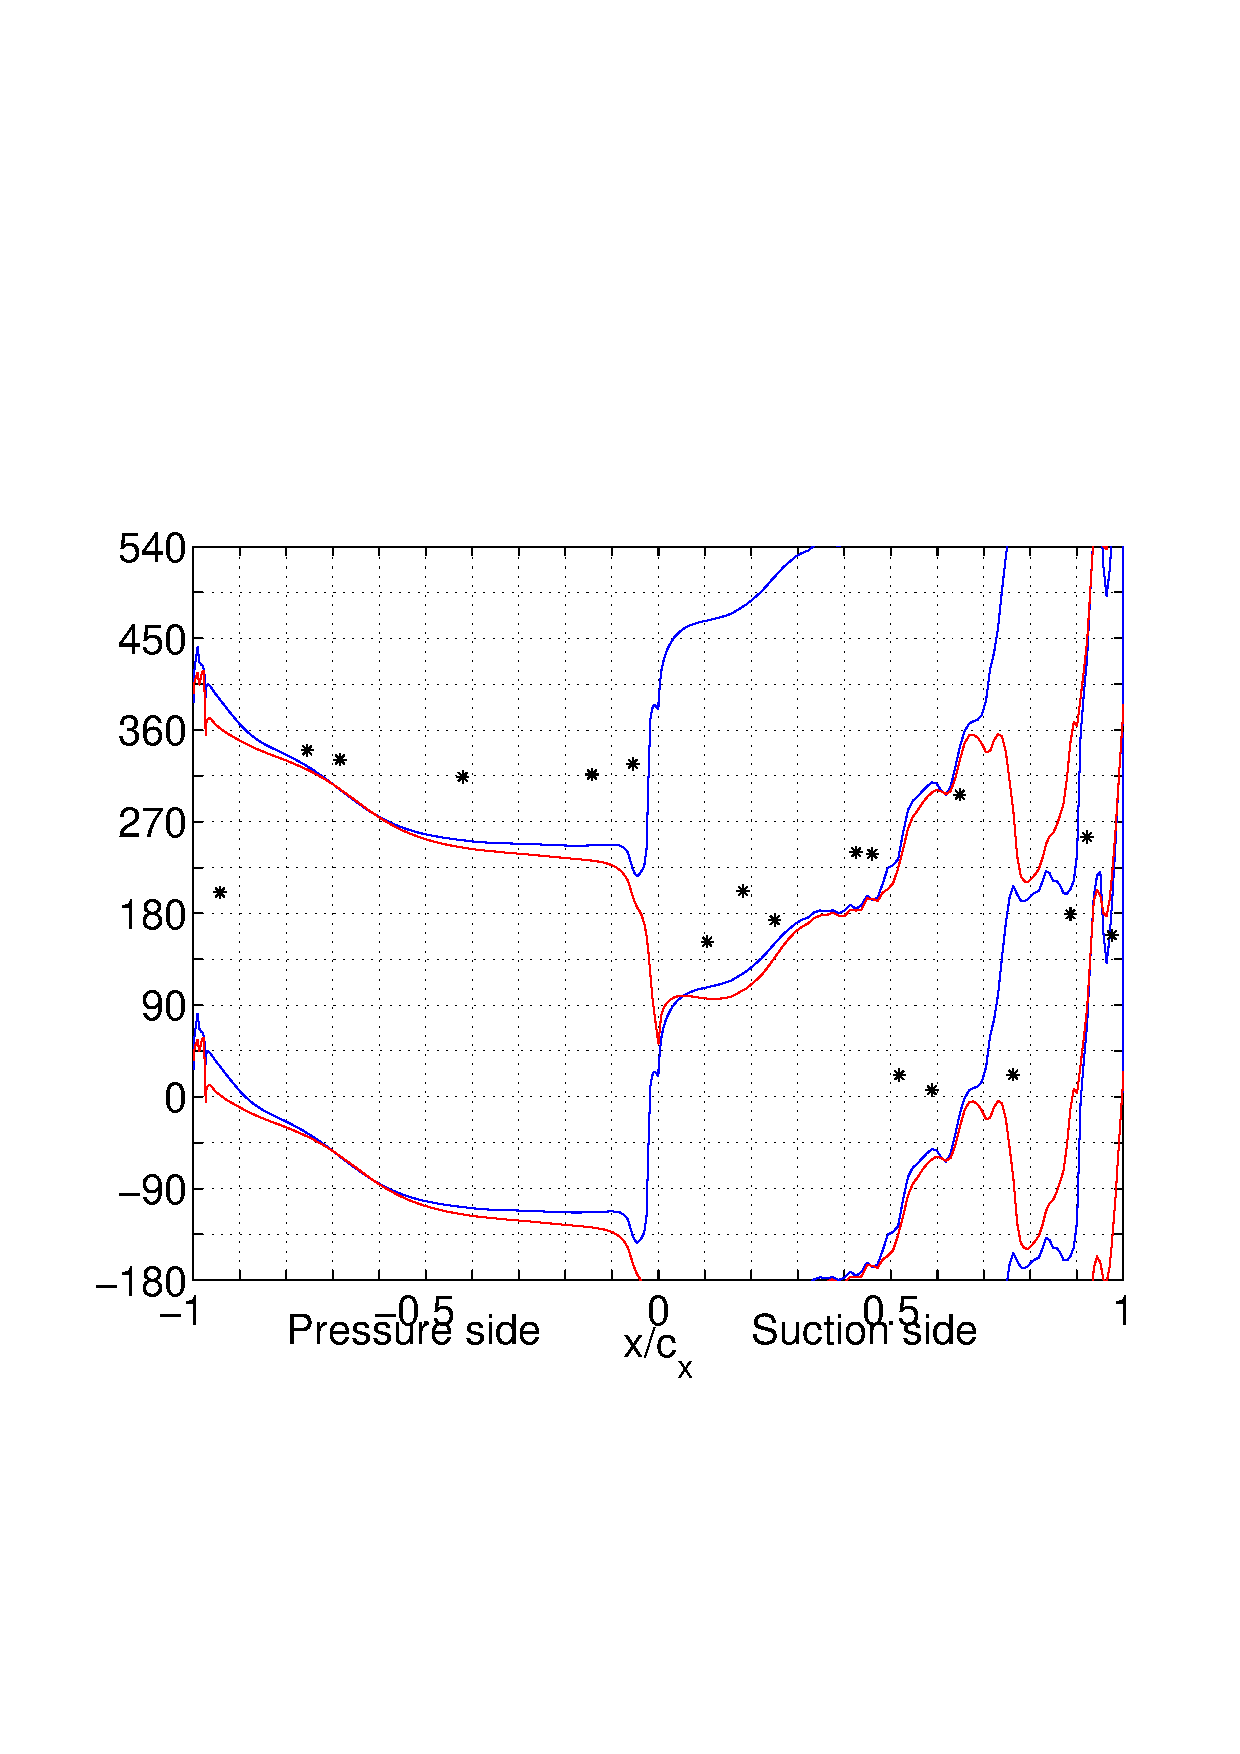
\includegraphics[width=75mm,clip=t]{CHAP_RT27/FIGURE/uns1pha2.pdf}}
   \end{tabular}
  \end{flushleft}
  \vspace{-8mm}
  \caption{RT27a rotor blade mid-section. Second Fourier component of
           dimensionless unsteady pressure.
           Linear method (blue),
           non-linear method (red) and
           measured data (stars).}
  \label{rt27_unsteady_2.fig}
\end{figure}
%
\begin{figure}
  \begin{flushleft}
   \begin{tabular}{ll}
     \subfigure[Amplitude of $\widetilde{p}/p_0$]
      {\hspace{-10mm}
       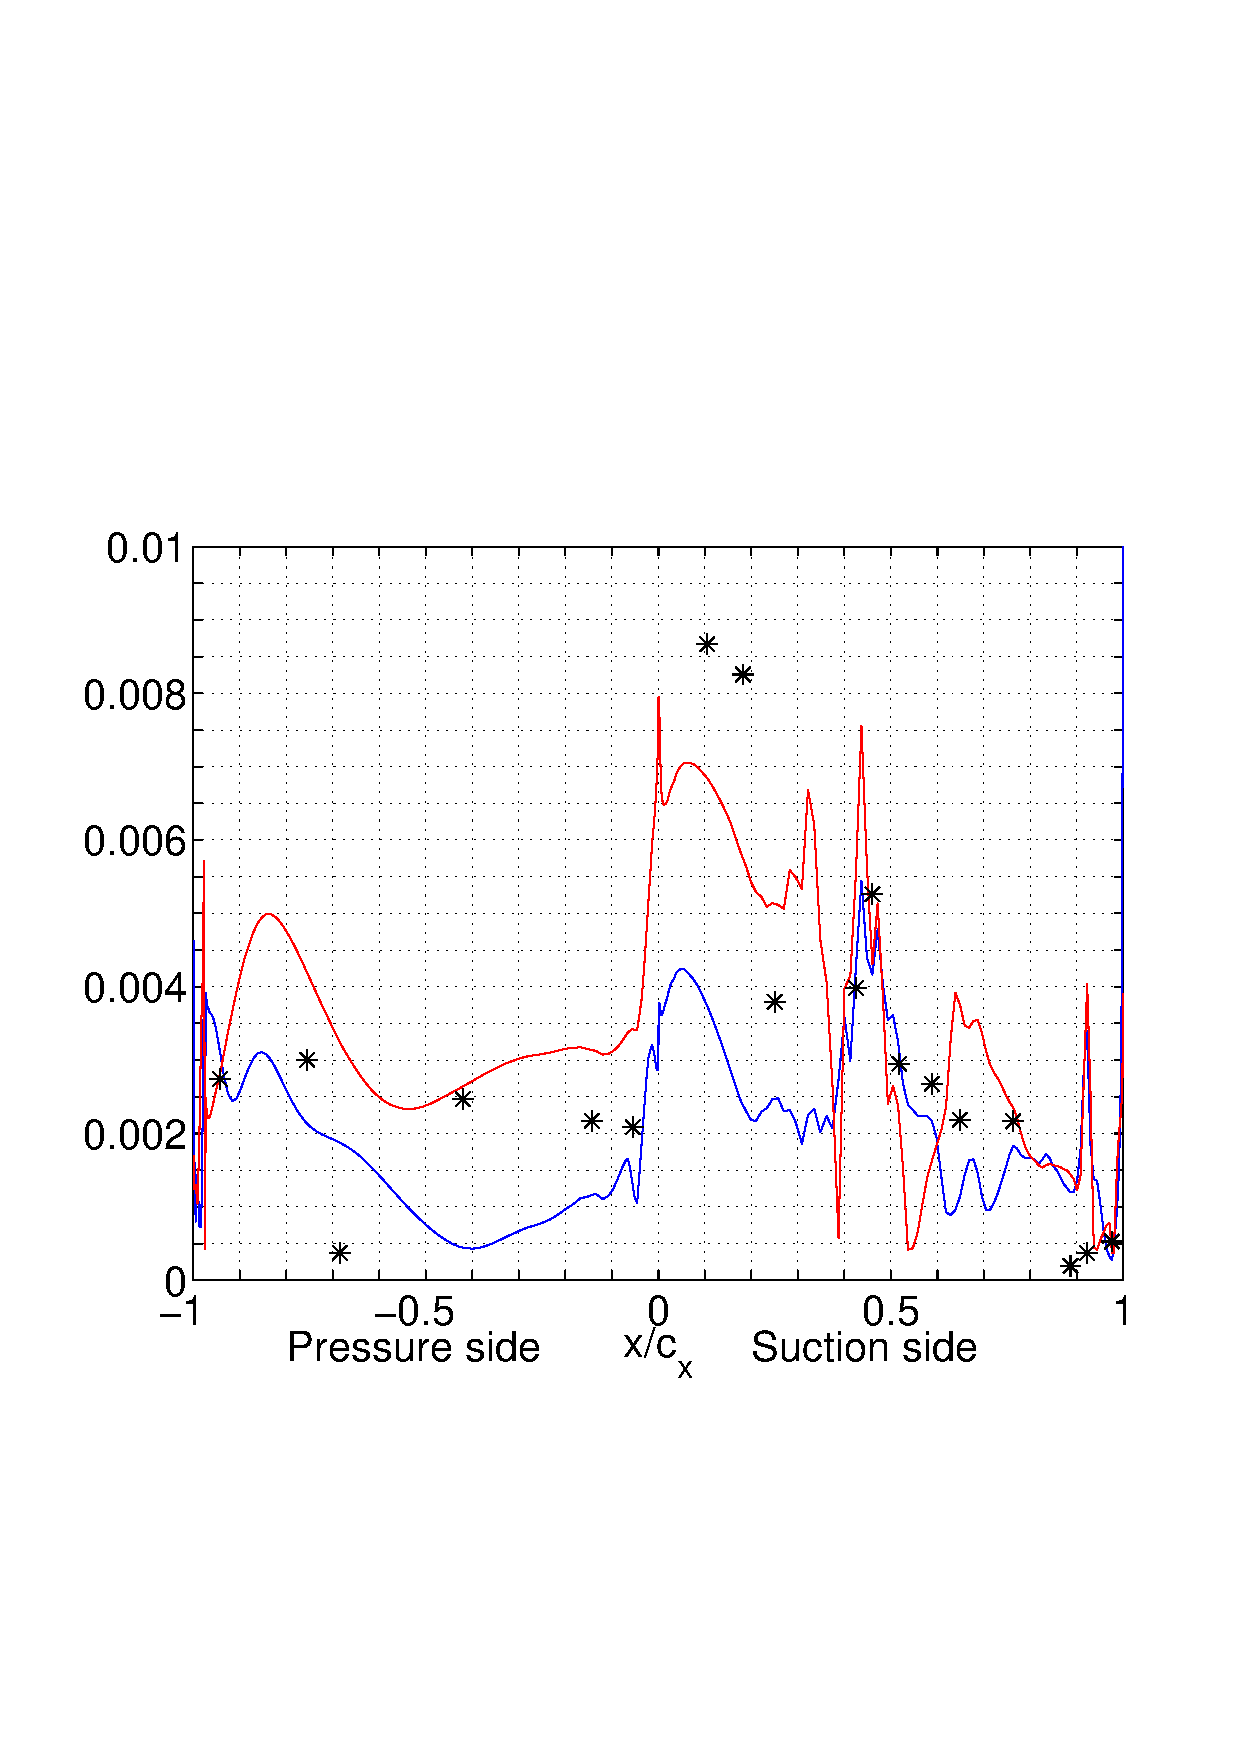
\includegraphics[width=75mm,clip=t]{CHAP_RT27/FIGURE/uns1amp3.pdf}}
         &
     \subfigure[Phase (deg)]
      {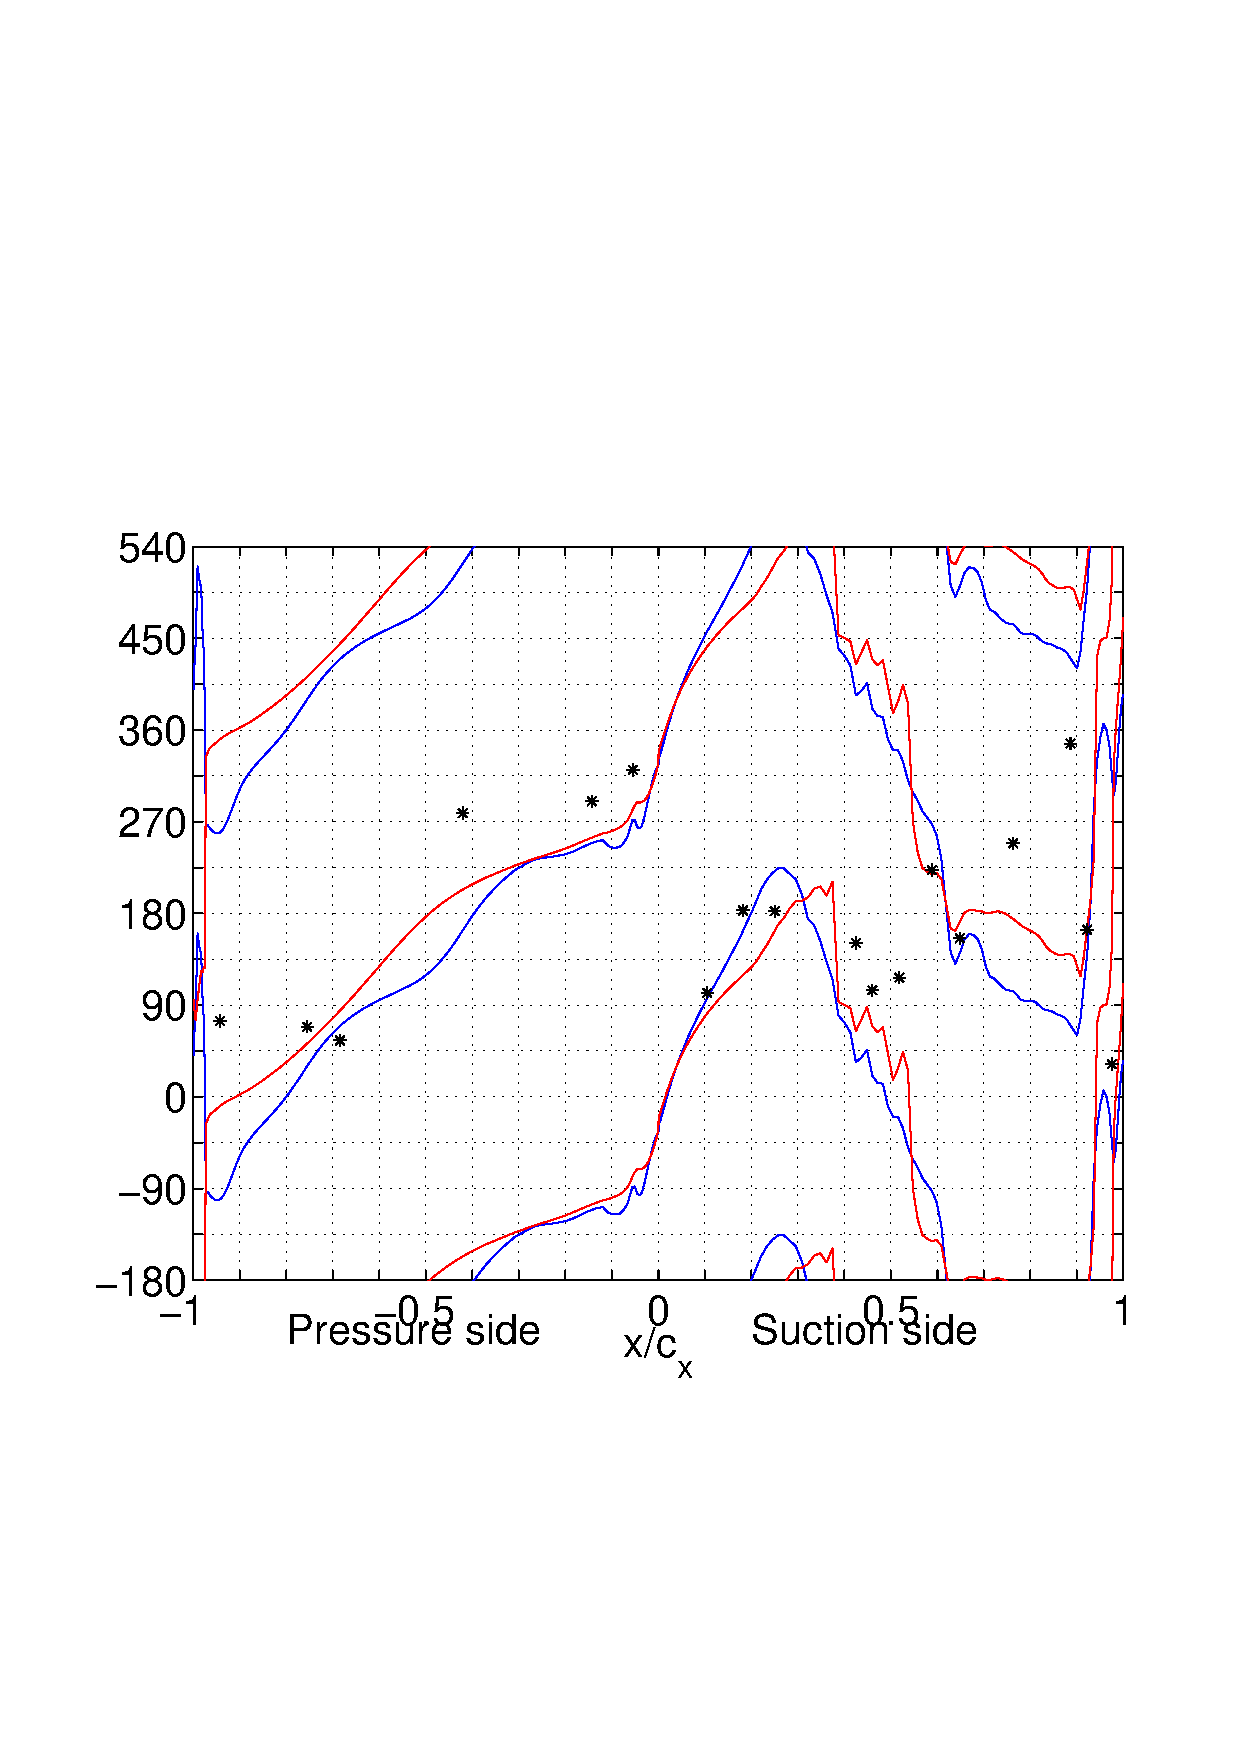
\includegraphics[width=75mm,clip=t]{CHAP_RT27/FIGURE/uns1pha3.pdf}}
   \end{tabular}
  \end{flushleft}
  \vspace{-8mm}
  \caption{RT27a rotor blade mid-section. Third Fourier component of
           dimensionless unsteady pressure.
           Linear method (blue),
           non-linear method (red) and
           measured data (stars).}
  \label{rt27_unsteady_3.fig}
\end{figure}
%
%
 The third Fourier component of the linear result underestimates
 by a factor of 50\% the non-linear results as shown in
 of Fig. \ref{rt27_unsteady_3.fig}. The phase still presents an overall
 good agreement.
 This discrepancy could be a direct consequence of two non-linear effects:
 (i) the steady-state NGV outlet solution underestimate the amplitude, for this
 particoular Fourier mode, of the time-averaged non-linear solution.
 This is evident in the leading-edge part ($0 < x/c\sm{x} < 0.3$)
 of rotor suction side of Fig. \ref{rt27_unsteady_3.fig}a.
 Infact, in this region the non-linear amplitude is higher then the linear
 one by a constant factor of $\approx 1.75$.
 (ii) Another cause of these discrepancies can be recover from the energy
 transfer between different Fourier modes.
 Although Fig. \ref{rt27_unsteady_3.fig}a evidentiates such non-linear
 features, it should be noted that the amplitude of this perturbancies
 is much lower than the those obtained for the first two Fourier modes
 of Figs. \ref{rt27_unsteady_1.fig} and \ref{rt27_unsteady_2.fig}.
%
%
%
\subsection{Reconstructed wave-forms}
%
 In this section the reconstructed wave forms over two blade passing cycles
 are reported. The waves are obtained by an inverse Fourier transform
 of the first three modes presented in Figs \ref{rt27_unsteady_1.fig},
 \ref{rt27_unsteady_2.fig} and \ref{rt27_unsteady_3.fig}.
 The position on the rotor blade surface of the various wave-forms
 is shown in Fig. \ref{rotor_mac_kul.fig}
%
%
